\documentclass[border=0.5cm]{standalone}
\usepackage{tikz}
\usetikzlibrary{positioning}

\begin{document}

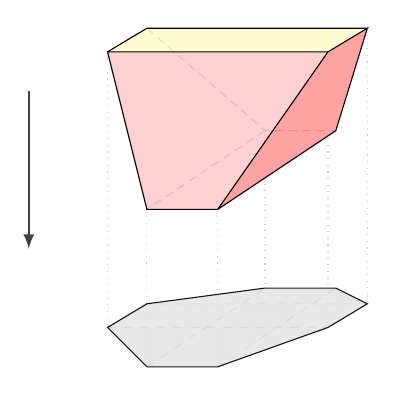
\begin{tikzpicture}
\coordinate (a1) at (0,0);
\coordinate (a2) at (2.8,0);
\coordinate (a3) at (3.3,.3);
\coordinate (a4) at (0.5,.3);
\coordinate (b1) at (0.5,-2);
\coordinate (b2) at (1.4,-2);
\coordinate (b3) at (2.9,-1);
\coordinate (b4) at (2,-1);
\draw[dotted,black!20] (a1) -- (0,-3.5) (a2) -- (2.8,-3.5) (b1) -- (0.5,-4) (b2) -- (1.4,-4) (a3) -- (3.3,-3.2) (b4) -- (2,-3);

\draw[thick,-latex,black!75] (-1,-0.5) -- (-1,-2.5);
\draw[black,densely dashed] (a4) -- (b4)--(b3)(b4) -- (b1);

\fill[red!20,opacity=0.9] (a1) -- (a2) --(b2) -- (b1) -- cycle;
\fill[red!40,opacity=0.9] (a2) -- (a3) --(b3) -- (b2) -- cycle;

\fill[yellow!20,opacity=0.9] (a2) -- (a3) --(a4) -- (a1) -- cycle;

\draw[black] (a1) -- (a2) -- (a3) -- (a4) -- (a1) -- (b1) -- (b2) -- (b3) -- (a3) -- (a2) -- (b2);


\coordinate (b11) at (0.5,-0.5);
\coordinate (b22) at (1.4,-0.5);
\coordinate (b33) at (2.9,0.5);
\coordinate (b44) at (2,0.5);
\begin{scope}[transform canvas={yshift = -3.5cm}]
\draw[gray, dashed] (a1) -- (a2)(a3) -- (a4)(b11) -- (b44)(b22) -- (b33);
\draw[fill =gray!20,opacity=0.9] (a1) -- (a4) -- (b44) -- (b33) -- (a3) -- (a2) -- (b22) -- (b11) -- cycle;
\end{scope}


\end{tikzpicture}


\end{document}
